\documentclass[a4paper,12pt]{article}

\usepackage[utf8]{inputenc}
\usepackage[T1]{polski}
\usepackage{helvet}
\usepackage{graphicx}
\usepackage{color}
\usepackage{xcolor}
\usepackage{geometry}
\usepackage{caption}
\usepackage{makeidx}
\usepackage{wrapfig}
\usepackage{listings}
\usepackage{hyperref}


\geometry{hmargin={2cm, 2cm}, height=10.0in}
\DeclareCaptionFont{white}{\color{white}}
\DeclareCaptionFormat{listing}{\colorbox{gray}{\parbox{\textwidth}{#1#2#3}}}
\captionsetup[lstlisting]{format=listing,labelfont=white,textfont=white}
\lstset{ %
language=Octave,                % choose the language of the code
basicstyle=\footnotesize,       % the size of the fonts that are used for the code
numbers=left,                   % where to put the line-numbers
numberstyle=\footnotesize,      % the size of the fonts that are used for the line-numbers
stepnumber=1,                   % the step between two line-numbers. If it's 1 each line 
                                % will be numbered
numbersep=5pt,                  % how far the line-numbers are from the code
backgroundcolor=\color{white},  % choose the background color. You must add \usepackage{color}
showspaces=false,               % show spaces adding particular underscores
showstringspaces=false,         % underline spaces within strings
showtabs=false,                 % show tabs within strings adding particular underscores
frame=single,	                % adds a frame around the code
tabsize=2,	                % sets default tabsize to 2 spaces
%captionpos=b,                   % sets the caption-position to bottom
breaklines=true,                % sets automatic line breaking
breakatwhitespace=false,        % sets if automatic breaks should only happen at whitespace
title=\lstname,                 % show the filename of files included with \lstinputlisting;
                                % also try caption instead of title
escapeinside={\%*}{*)},         % if you want to add a comment within your code
morekeywords={*,...}            % if you want to add more keywords to the set
}

\lstloadlanguages{ Ruby }


\makeindex

\begin{document}

% =====  STRONA TYTULOWA PRACY INŻYNIERSKIEJ ====
% ostatnia modyfikacja: 2009/07/01, K. Malarz

\thispagestyle{empty}

%% ------------------------ NAGLOWEK STRONY ---------------------------------
\begin{figure}
\vspace{-13cm}
\hspace{-4cm}

\includegraphics[height=29.3cm]{grafika/agh_nzw_a_pl_1w_wbr_cmyk.pdf}\\
\vspace{-13.9cm}
\end{figure}
\rule{26mm}{0pt}
{\large\textsf{Wydział Fizyki i Informatyki Stosowanej}}\\
\rule{\textwidth}{3pt}\\
\rule[2ex]
{\textwidth}{1pt}\\
\vspace{7ex}
\begin{center}
{\bf\LARGE\textsf{Analiza i przetwarzanie obrazów}}\\
\vspace{13ex}
{\bf\huge\textsf{Ćwiczenie 5}}\\
\vspace{3ex}
{\sf \small } {\bf\small\textsf{Krystian Wojtas}}\\
\vspace{14ex}
%% ------------------------ OPIEKUN PRACY ------------------------------------
{\sf \Large } {\bf\Large\textsf{}}\\
\vspace{22ex}
\textsf{\bf\large\textsf{Kraków, grudzień 2011}}
\end{center}
%% =====  STRONA TYTUŁOWA PRACY INŻYNIERSKIEJ  ====


\newpage
\section{Wstęp}
Celem ćwiczeń było ścienianie i szkieletyzacja obrazka. Wykorzystany został język Ruby i jego framework RMagic, który binduje funkcje biblioteczne z pakietu ImageMagick.


\subsection{Definicje}

\subsubsection{Ścienianie}
\begin{quote}
Ścienianie to nazwa grupy przekształceń morfologicznych, których działanie polega na:

- przykładaniu elementu strukturalnego do kolejnych punktów obrazu,

- zmianie wartości punktu na 0, gdy element strukturalny pasuje do przyłożonego miejsca,

- w przypadku braku zgodności wartość punktu pozostaje bez zmian.

W większości przypadków element strukturalny jest rotowany (obracany o 90 stopni) pomiędzy kolejnymi operacjami. Ścienianie może być powtarzane, aż do momentu, w którym kolejne powtórzenie operacji nie wprowadza żadnych zmian. Cechą charakterystyczną dla przekształceń z grupy ścieniania jest to, że figury uzyskane po ścienianiu zawierają się w całości w figurach wyjściowych. 
\end{quote}
Źródło \url{http://atol.am.gdynia.pl/tc/Radzienski/scienianie.htm}

\subsubsection{Szkieletyzacja}
\begin{quote}
Szkieletyzacja jest operacją pozwalającą wyodrębnić osiowe punkty
(szkielety) w analizowanym obrazie.

Szkielet figury jest zbiorem wszystkich punktów, które są
równoodległe od co najmniej dwóch punktów należących
do brzegu.

Szkielet figury jest znacznie od niej mniejszy, a odzwierciedla w pełni jej
topologiczne własności.
\end{quote}
Źródło \url{http://aragorn.pb.bialystok.pl/~boldak/DIP/CPO-W05-v01-50pr.pdf}


\section{Maska}

\lstinputlisting[caption=Implementacja algorytmu scieniania przez maske]{listingi/scienianie.rb}

\section{KMM}

\lstinputlisting[caption=Implementacja algorytmu KMM]{listingi/kmm.rb}


\section{Wyniki}

\subsection{p1}

\begin{figure}[h!]
\begin{minipage}[t]{7.5cm}
\begin{center}
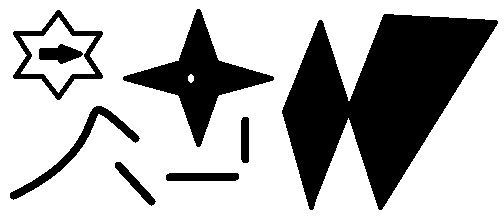
\includegraphics[width=7.5cm]{../in/p1.jpg}
\caption{orginal}
\end{center}
\end{minipage}
\hfill
\begin{minipage}[t]{7.5cm}
\begin{center}
\includegraphics[width=7.5cm]{../out/sc_p1_100.jpg}
\caption{ścienianie, 54 iteracji}
\end{center}
\end{minipage}
\end{figure}

\begin{figure}[h!]
\begin{minipage}[t]{7.5cm}
\begin{center}
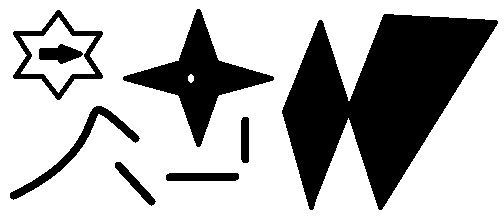
\includegraphics[width=7.5cm]{../in/p1.jpg}
\caption{orginal}
\end{center}
\end{minipage}
\hfill
\begin{minipage}[t]{7.5cm}
\begin{center}
\includegraphics[width=7.5cm]{../out/kmm_p1_100.jpg}
\caption{kmm, 34 iteracji}
\end{center}
\end{minipage}
\end{figure}

\begin{figure}[h!]
\begin{minipage}[t]{5cm}
\begin{center}
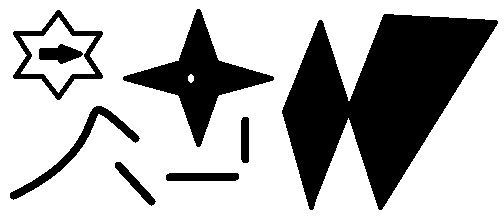
\includegraphics[width=5cm]{../in/p1.jpg}
\caption{orginal}
\end{center}
\end{minipage}
\hfill
\begin{minipage}[t]{5cm}
\begin{center}
\includegraphics[width=5cm]{../out/sc_p1_100.jpg}
\caption{ścienianie, 54 iteracji}
\end{center}
\end{minipage}
\hfill
\begin{minipage}[t]{5cm}
\begin{center}
\includegraphics[width=5cm]{../out/kmm_p1_100.jpg}
\caption{kmm, 34 iteracji}
\end{center}
\end{minipage}
\end{figure}



\newpage
\subsection{p2}

\begin{figure}[h!]
\begin{minipage}[t]{7.5cm}
\begin{center}
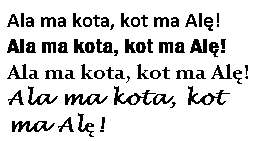
\includegraphics[width=7.5cm]{../in/p2.jpg}
\caption{orginal}
\end{center}
\end{minipage}
\hfill
\begin{minipage}[t]{7.5cm}
\begin{center}
\includegraphics[width=7.5cm]{../out/sc_p2_100.jpg}
\caption{ścienianie, 4 iteracje}
\end{center}
\end{minipage}
\end{figure}

\begin{figure}[h!]
\begin{minipage}[t]{7.5cm}
\begin{center}
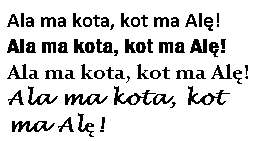
\includegraphics[width=7.5cm]{../in/p2.jpg}
\caption{orginal}
\end{center}
\end{minipage}
\hfill
\begin{minipage}[t]{7.5cm}
\begin{center}
\includegraphics[width=7.5cm]{../out/kmm_p2_100.jpg}
\caption{kmm, 4 iteracje}
\end{center}
\end{minipage}
\end{figure}

\begin{figure}[h!]
\begin{minipage}[t]{5cm}
\begin{center}
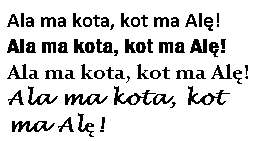
\includegraphics[width=5cm]{../in/p2.jpg}
\caption{orginal}
\end{center}
\end{minipage}
\hfill
\begin{minipage}[t]{5cm}
\begin{center}
\includegraphics[width=5cm]{../out/sc_p2_100.jpg}
\caption{ścienianie, 4 iteracje}
\end{center}
\end{minipage}
\hfill
\begin{minipage}[t]{5cm}
\begin{center}
\includegraphics[width=5cm]{../out/kmm_p2_100.jpg}
\caption{kmm, 4 iteracje}
\end{center}
\end{minipage}
\end{figure}



\newpage
\subsection{p3}

\begin{figure}[h!]
\begin{minipage}[t]{7.5cm}
\begin{center}
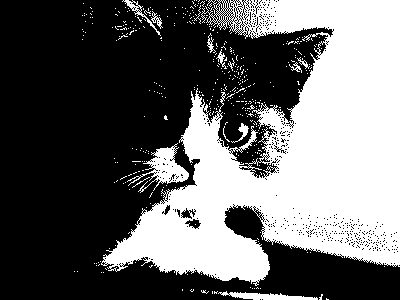
\includegraphics[width=7.5cm]{../in/p3.jpg}
\caption{orginal}
\end{center}
\end{minipage}
\hfill
\begin{minipage}[t]{7.5cm}
\begin{center}
\includegraphics[width=7.5cm]{../out/sc_p3_100.jpg}
\caption{ścienianie, 76 iteracji}
\end{center}
\end{minipage}
\end{figure}

\begin{figure}[h!]
\begin{minipage}[t]{7.5cm}
\begin{center}
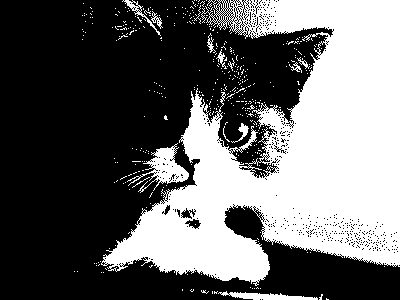
\includegraphics[width=7.5cm]{../in/p3.jpg}
\caption{orginal}
\end{center}
\end{minipage}
\hfill
\begin{minipage}[t]{7.5cm}
\begin{center}
\includegraphics[width=7.5cm]{../out/kmm_p3_100.jpg}
\caption{kmm, 60 iteracji}
\end{center}
\end{minipage}
\end{figure}

\begin{figure}[h!]
\begin{minipage}[t]{5cm}
\begin{center}
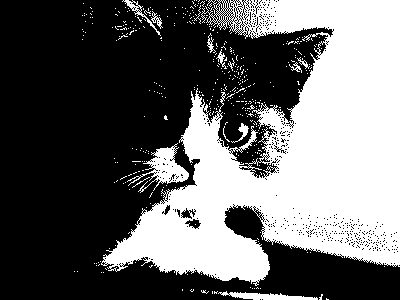
\includegraphics[width=5cm]{../in/p3.jpg}
\caption{orginal}
\end{center}
\end{minipage}
\hfill
\begin{minipage}[t]{5cm}
\begin{center}
\includegraphics[width=5cm]{../out/sc_p3_100.jpg}
\caption{ścienianie, 76 iteracji}
\end{center}
\end{minipage}
\hfill
\begin{minipage}[t]{5cm}
\begin{center}
\includegraphics[width=5cm]{../out/kmm_p3_100.jpg}
\caption{kmm, 60 iteracji}
\end{center}
\end{minipage}
\end{figure}



\newpage
\subsection{p4}

\begin{figure}[h!]
\begin{minipage}[t]{7.5cm}
\begin{center}
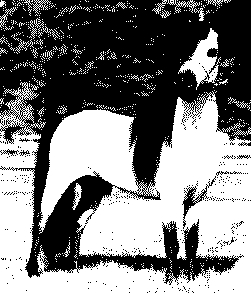
\includegraphics[width=7.5cm]{../in/p4.jpg}
\caption{orginal}
\end{center}
\end{minipage}
\hfill
\begin{minipage}[t]{7.5cm}
\begin{center}
\includegraphics[width=7.5cm]{../out/sc_p4_100.jpg}
\caption{ścienianie, 22 iteracji}
\end{center}
\end{minipage}
\end{figure}

\begin{figure}[h!]
\begin{minipage}[t]{7.5cm}
\begin{center}
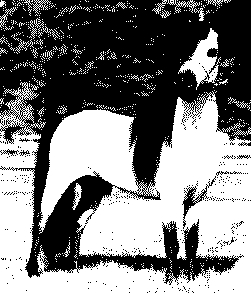
\includegraphics[width=7.5cm]{../in/p4.jpg}
\caption{orginal}
\end{center}
\end{minipage}
\hfill
\begin{minipage}[t]{7.5cm}
\begin{center}
\includegraphics[width=7.5cm]{../out/kmm_p4_100.jpg}
\caption{kmm, 19 iteracji}
\end{center}
\end{minipage}
\end{figure}

\begin{figure}[h!]
\begin{minipage}[t]{5cm}
\begin{center}
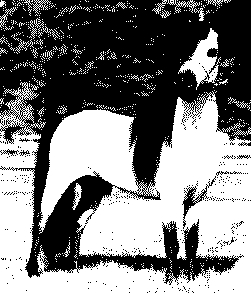
\includegraphics[width=5cm]{../in/p4.jpg}
\caption{orginal}
\end{center}
\end{minipage}
\hfill
\begin{minipage}[t]{5cm}
\begin{center}
\includegraphics[width=5cm]{../out/sc_p4_100.jpg}
\caption{ścienianie, 22 iteracji}
\end{center}
\end{minipage}
\hfill
\begin{minipage}[t]{5cm}
\begin{center}
\includegraphics[width=5cm]{../out/kmm_p4_100.jpg}
\caption{kmm, 19 iteracji}
\end{center}
\end{minipage}
\end{figure}



\newpage
\subsection{o1}

\begin{figure}[h!]
\begin{minipage}[t]{7.5cm}
\begin{center}

\includegraphics[width=7.5cm]{../in/o1.jpg}
\caption{orginal}
\end{center}
\end{minipage}
\hfill
\begin{minipage}[t]{7.5cm}
\begin{center}
\includegraphics[width=7.5cm]{../out/sc_o1_100.jpg}
\caption{ścienianie, 47 iteracji}
\end{center}
\end{minipage}
\end{figure}

\begin{figure}[h!]
\begin{minipage}[t]{7.5cm}
\begin{center}

\includegraphics[width=7.5cm]{../in/o1.jpg}
\caption{orginal}
\end{center}
\end{minipage}
\hfill
\begin{minipage}[t]{7.5cm}
\begin{center}
\includegraphics[width=7.5cm]{../out/kmm_o1_100.jpg}
\caption{kmm, 37 iteracji}
\end{center}
\end{minipage}
\end{figure}

\begin{figure}[h!]
\begin{minipage}[t]{5cm}
\begin{center}

\includegraphics[width=5cm]{../in/o1.jpg}
\caption{orginal}
\end{center}
\end{minipage}
\hfill
\begin{minipage}[t]{5cm}
\begin{center}
\includegraphics[width=5cm]{../out/sc_o1_100.jpg}
\caption{ścienianie, 47 iteracji}
\end{center}
\end{minipage}
\hfill
\begin{minipage}[t]{5cm}
\begin{center}
\includegraphics[width=5cm]{../out/kmm_o1_100.jpg}
\caption{kmm, 37 iteracji}
\end{center}
\end{minipage}
\end{figure}



\newpage
\subsection{o2}

\begin{figure}[h!]
\begin{minipage}[t]{7.5cm}
\begin{center}
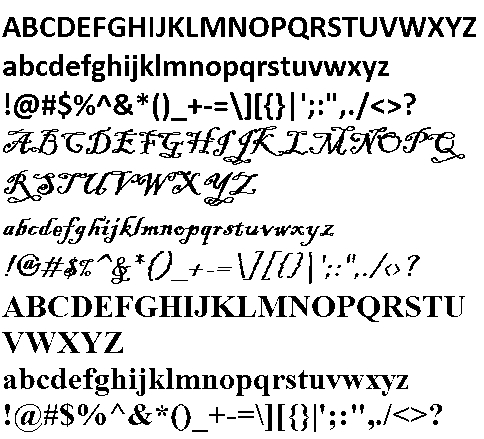
\includegraphics[width=7.5cm]{../in/o2.jpg}
\caption{orginal}
\end{center}
\end{minipage}
\hfill
\begin{minipage}[t]{7.5cm}
\begin{center}
\includegraphics[width=7.5cm]{../out/sc_o2_100.jpg}
\caption{ścienianie, 4 iteracje}
\end{center}
\end{minipage}
\end{figure}

\begin{figure}[h!]
\begin{minipage}[t]{7.5cm}
\begin{center}
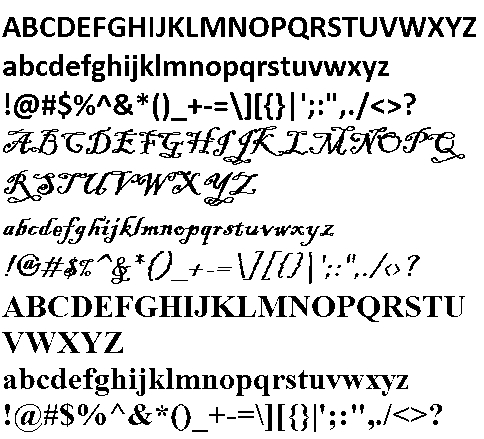
\includegraphics[width=7.5cm]{../in/o2.jpg}
\caption{orginal}
\end{center}
\end{minipage}
\hfill
\begin{minipage}[t]{7.5cm}
\begin{center}
\includegraphics[width=7.5cm]{../out/kmm_o2_100.jpg}
\caption{kmm, 4 iteracje}
\end{center}
\end{minipage}
\end{figure}

\begin{figure}[h!]
\begin{minipage}[t]{5cm}
\begin{center}
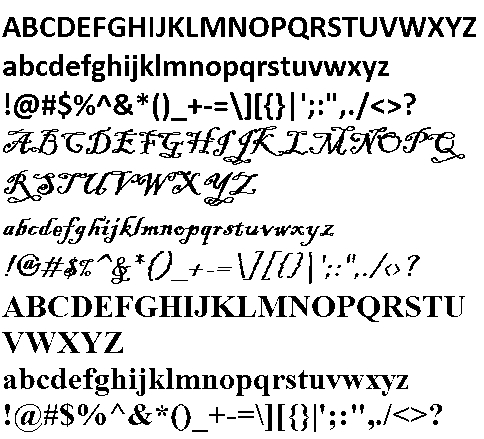
\includegraphics[width=5cm]{../in/o2.jpg}
\caption{orginal}
\end{center}
\end{minipage}
\hfill
\begin{minipage}[t]{5cm}
\begin{center}
\includegraphics[width=5cm]{../out/sc_o2_100.jpg}
\caption{ścienianie, 4 iteracje}
\end{center}
\end{minipage}
\hfill
\begin{minipage}[t]{5cm}
\begin{center}	
\includegraphics[width=5cm]{../out/kmm_o2_100.jpg}
\caption{kmm, 4 iteracje}	
\end{center}
\end{minipage}
\end{figure}


\newpage	
\section{Wnioski}
Algorytm KMM wytwarza wyraźnie lepsze rezultaty, metoda maski wytwarza szkielety poszarpane.

Algorytmom najwięcej pracy zajmuje zeszkieletyzowanie obszarów wypełnionych jednolitą czernią. Są to wypełnione figury lub plamy czarnego tła. Najszybciej zbieżne są elementy wąskie jak litery.

KMM wykonuje mniej iteracji lub przynajmniej tyle samo przy wąskich figurach. 

\end{document}
